\section[Analysis]{Analysis}
\begin{frame}
\frametitle{Objectives}
\begin{block}{Objective}
\begin{itemize}
\item
Estimate masses, dimensions
\item
Choose motors and electronics
\end{itemize}
\end{block}

\begin{columns}
\uncover<1->{
\column{0.5\textwidth}
\vspace*{0.2in}
\begin{block}{Design 1}
\end{block}
\begin{itemize}
\item
Reaction wheel
\item
Springs
\item
Winding motor
\item
Platform
\item
\alert{ Lower leg, main leg masses}
\end{itemize}
}
\uncover<2->{
\column{0.5\textwidth}
\begin{block}{Design 2}
\end{block}
\begin{itemize}
\item
Reaction wheel
\item
Springs
\item
\alert{Rack-pinion drive and motor}
\item
Platform and leg mass
\end{itemize}
}
\end{columns}
\end{frame}

\subsection*{Two Mass Problem}
\begin{frame}
\frametitle{Two Mass Problem}

\begin{columns}
\column{0.4\textwidth}

\begin{tikzpicture}[scale=0.45]
\draw (-3,0) -- (3,0);
\foreach \x in {-2.5,-2,...,2.5}
\draw (\x,0) -- (\x+0.5,-0.5);
\path (-2,7) coordinate(M1);
\path (2,10) coordinate(M2);
\path (-0.6,2) coordinate(m1);
\path (0.6,3.2) coordinate(m2);
\draw [thick](M1) rectangle (M2) node[midway]{\huge{$M$}};
\draw [thick](m1) rectangle (m2) node[midway]{\Large{$m$}};
\path (-2.5,0) coordinate (O);
\path (-2.5,2.6) coordinate (SPL);
\path (-2.5,8.5) coordinate (H);
\draw[<->] [semithick](O)++(-0.5,0) -- (-3,8.5) node[midway, left]{$H$};
\draw[<->] [semithick](SPL) -- (H) node[midway, right]{$l_0$};
\draw[snake=coil, segment amplitude=8pt] (0,3.2) -- (0,7) node[midway,right=2ex]{$k$};
\end{tikzpicture}

\column{0.6\textwidth}
\uncover<1->{
\begin{itemize}
\item
\begin{equation*}
h_n = \frac{Mh_{n-1} + ml_0}{M + m}
\end{equation*}
\item
\begin{equation*}
E_{loss} = \frac{Mg\;(H-l_0)}{1 + M/m}
\end{equation*}
\end{itemize}
}

\visible<2->{
\begin{figure}
\centering
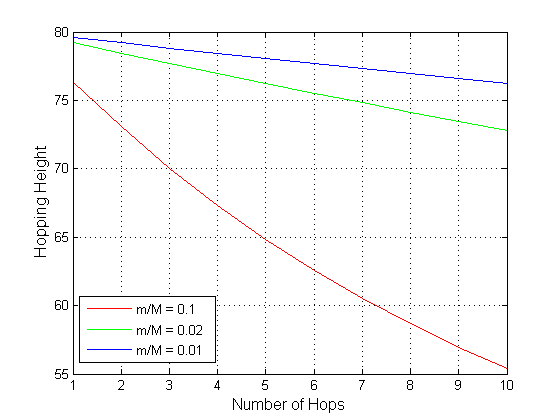
\includegraphics[scale=0.4]{fig/hopHeight.png}
\end{figure}
}
\end{columns}

\end{frame}

\begin{frame}
\frametitle{Torque Requirements}
\begin{columns}
\column{0.7\textwidth}
\begin{figure}
\centering
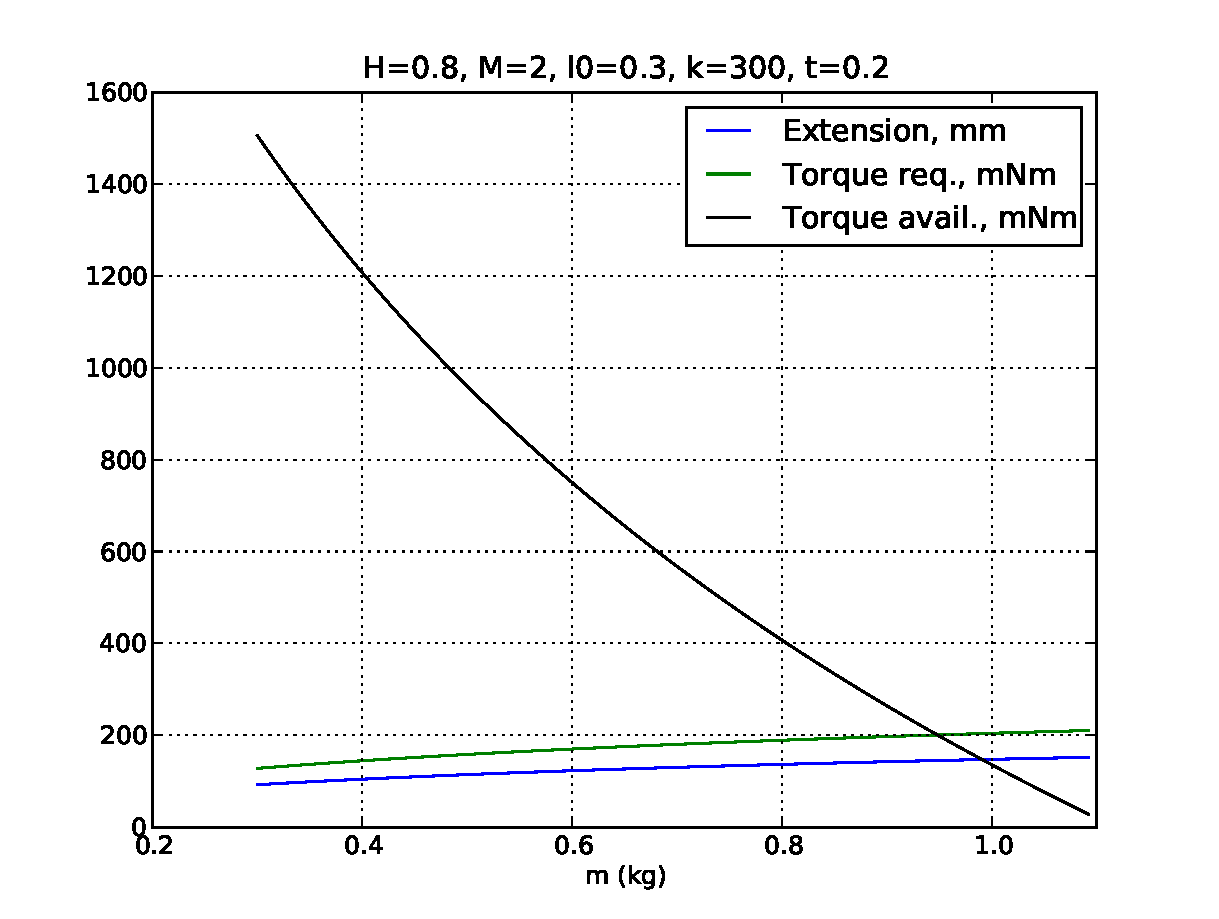
\includegraphics[width=\textwidth]{fig/2mass.pdf}
\end{figure}

\column{0.4\textwidth}
\visible<2->{
\begin{block}{Results}
\begin{itemize}
\item
m $\sim$ 0.5 kg
\item
k $\sim$ 300 N
\item
M $\sim$ 2 kg
\item
Lower leg $\sim$ 12 cms
\item
Standard rack-pinion
\item
Faulhabeur 2342 motor
\item
43 : 1 gearbox
\end{itemize}
\end{block}
}
\end{columns}
\end{frame}


\subsection*{Reaction Wheel}
\begin{frame}
\frametitle{ReWac : Idea and Advantages}
\begin{columns}

\column{0.4\textwidth}
\begin{figure}
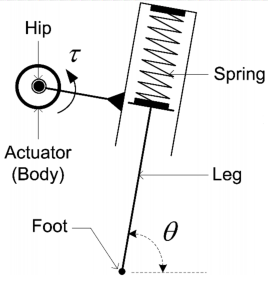
\includegraphics[width=\textwidth]{fig/slom.pdf}
\caption{ReWac : Schematic}
\end{figure}

\column{0.6\textwidth}
\begin{block}{Inertia Wheel Assembly}
Conserve angular momentum
\begin{equation*}
\dot{\theta}_b = -\frac{J_{w}}{J_{b}+J_{w}}\dot{\theta}_w
\end{equation*}
\end{block}

\vspace{0.5in}
\begin{block}{Uses}
\begin{itemize}
\item
Initial condition\\[0.1in]
\item
Changing hopping height online\\[0.1in]
\item
Change from an \alert{arbitrary} pitch to \alert{steady state} pitch
within one hop
\end{itemize}
\end{block}
\end{columns}

\end{frame}

\begin{frame}
\frametitle{ReWac : Radius}
\begin{figure}
\centering
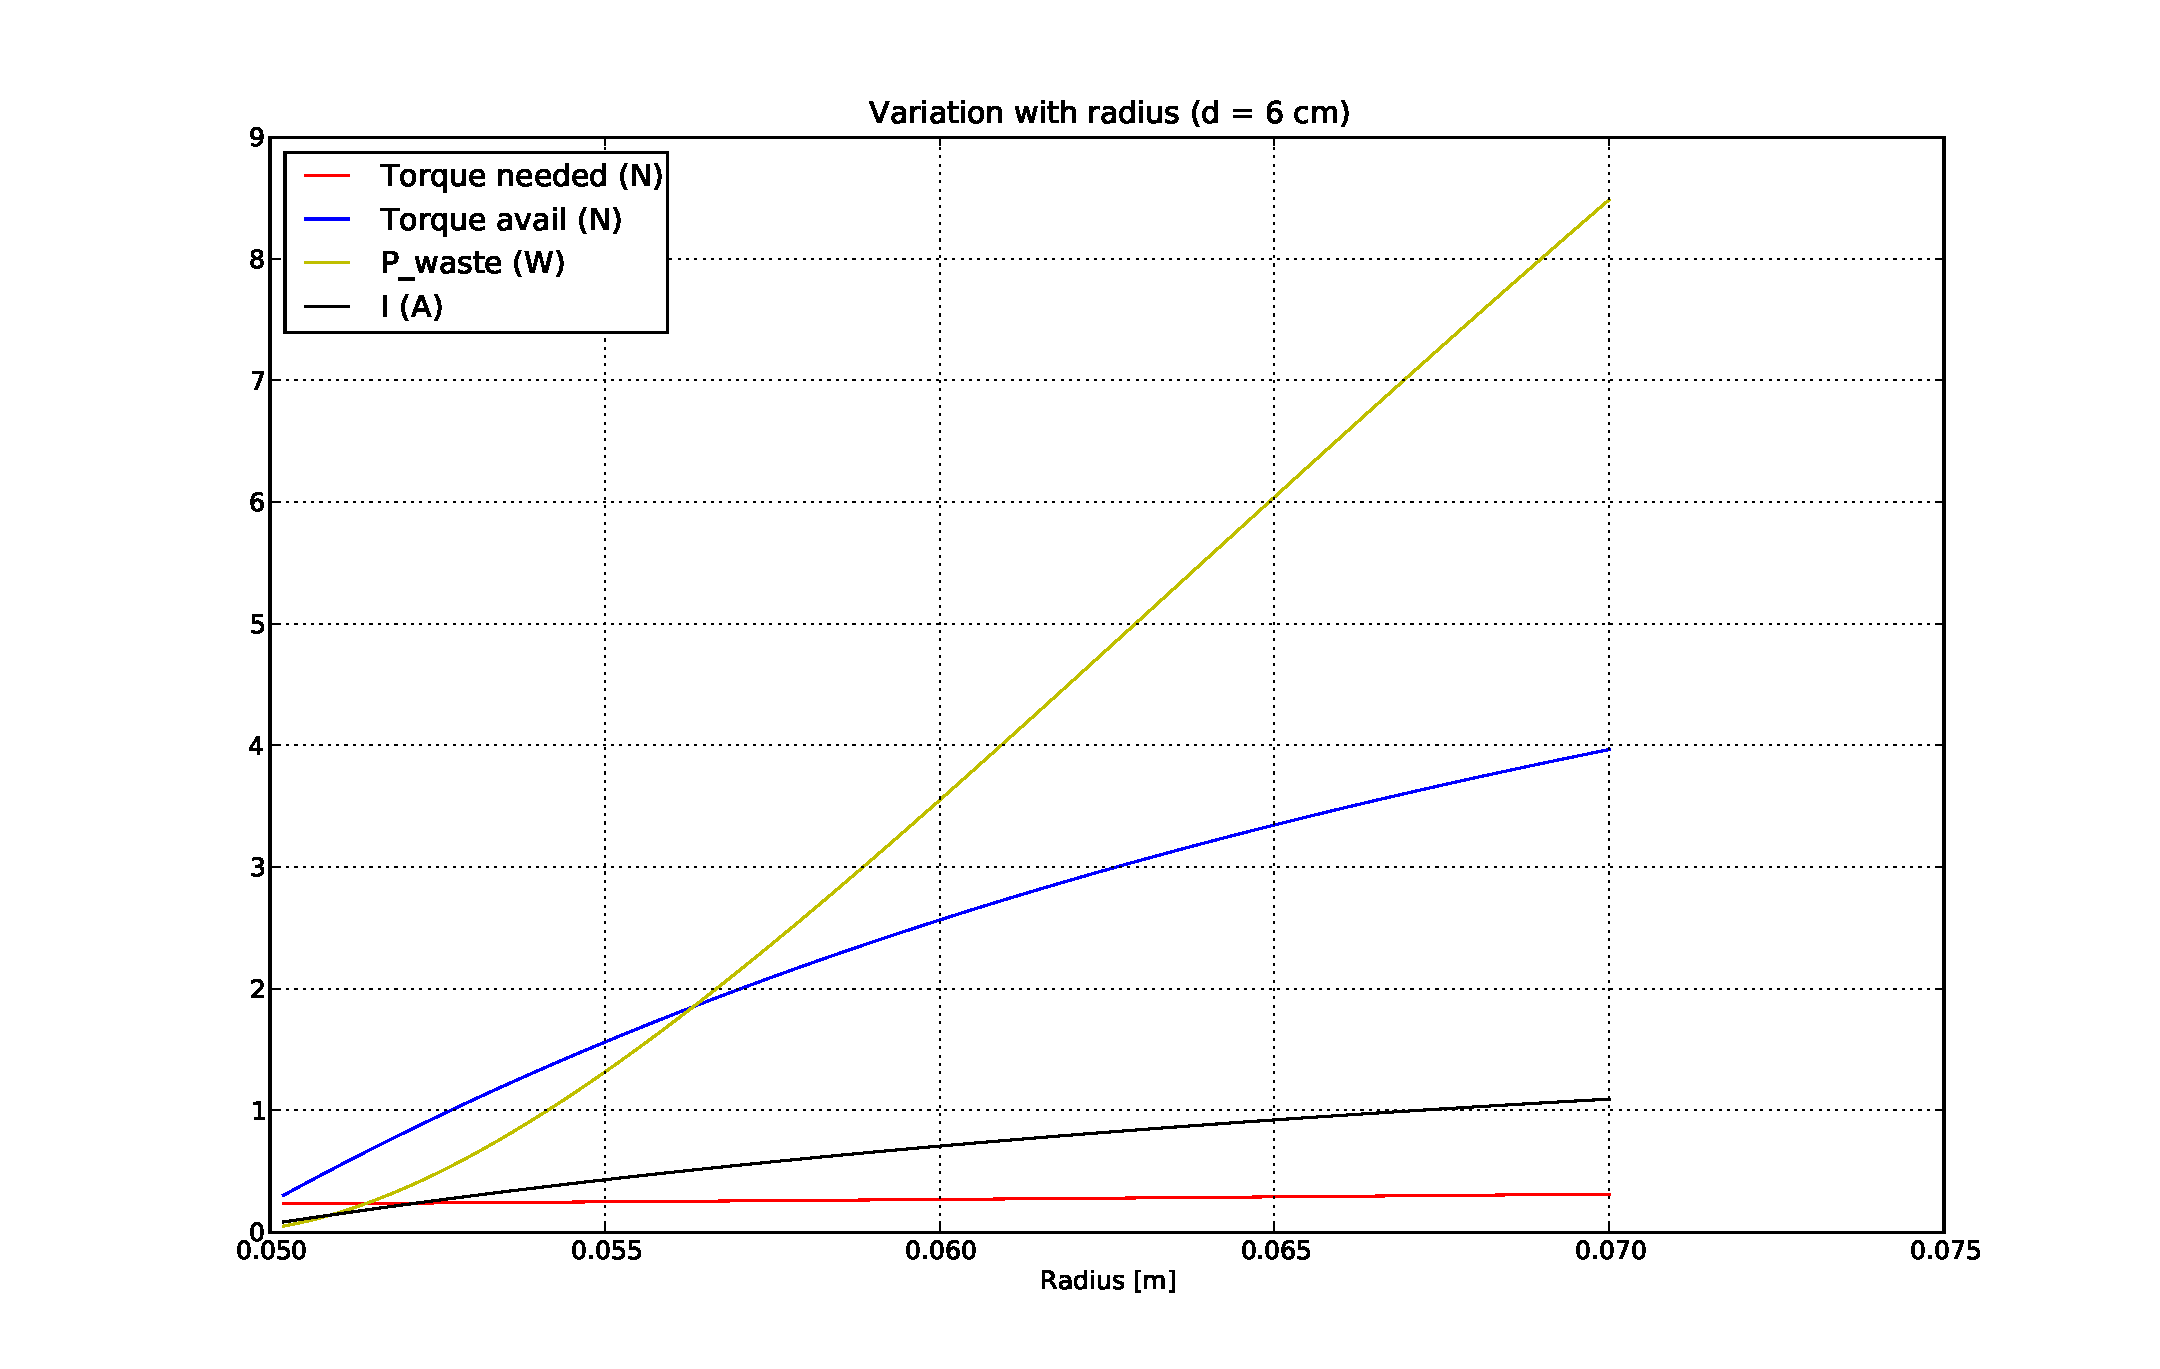
\includegraphics[width=\textwidth]{fig/rewac_radius.pdf}
\end{figure}
\end{frame}

\begin{frame}
\frametitle{ReWac : CG distance}
\begin{figure}
\centering
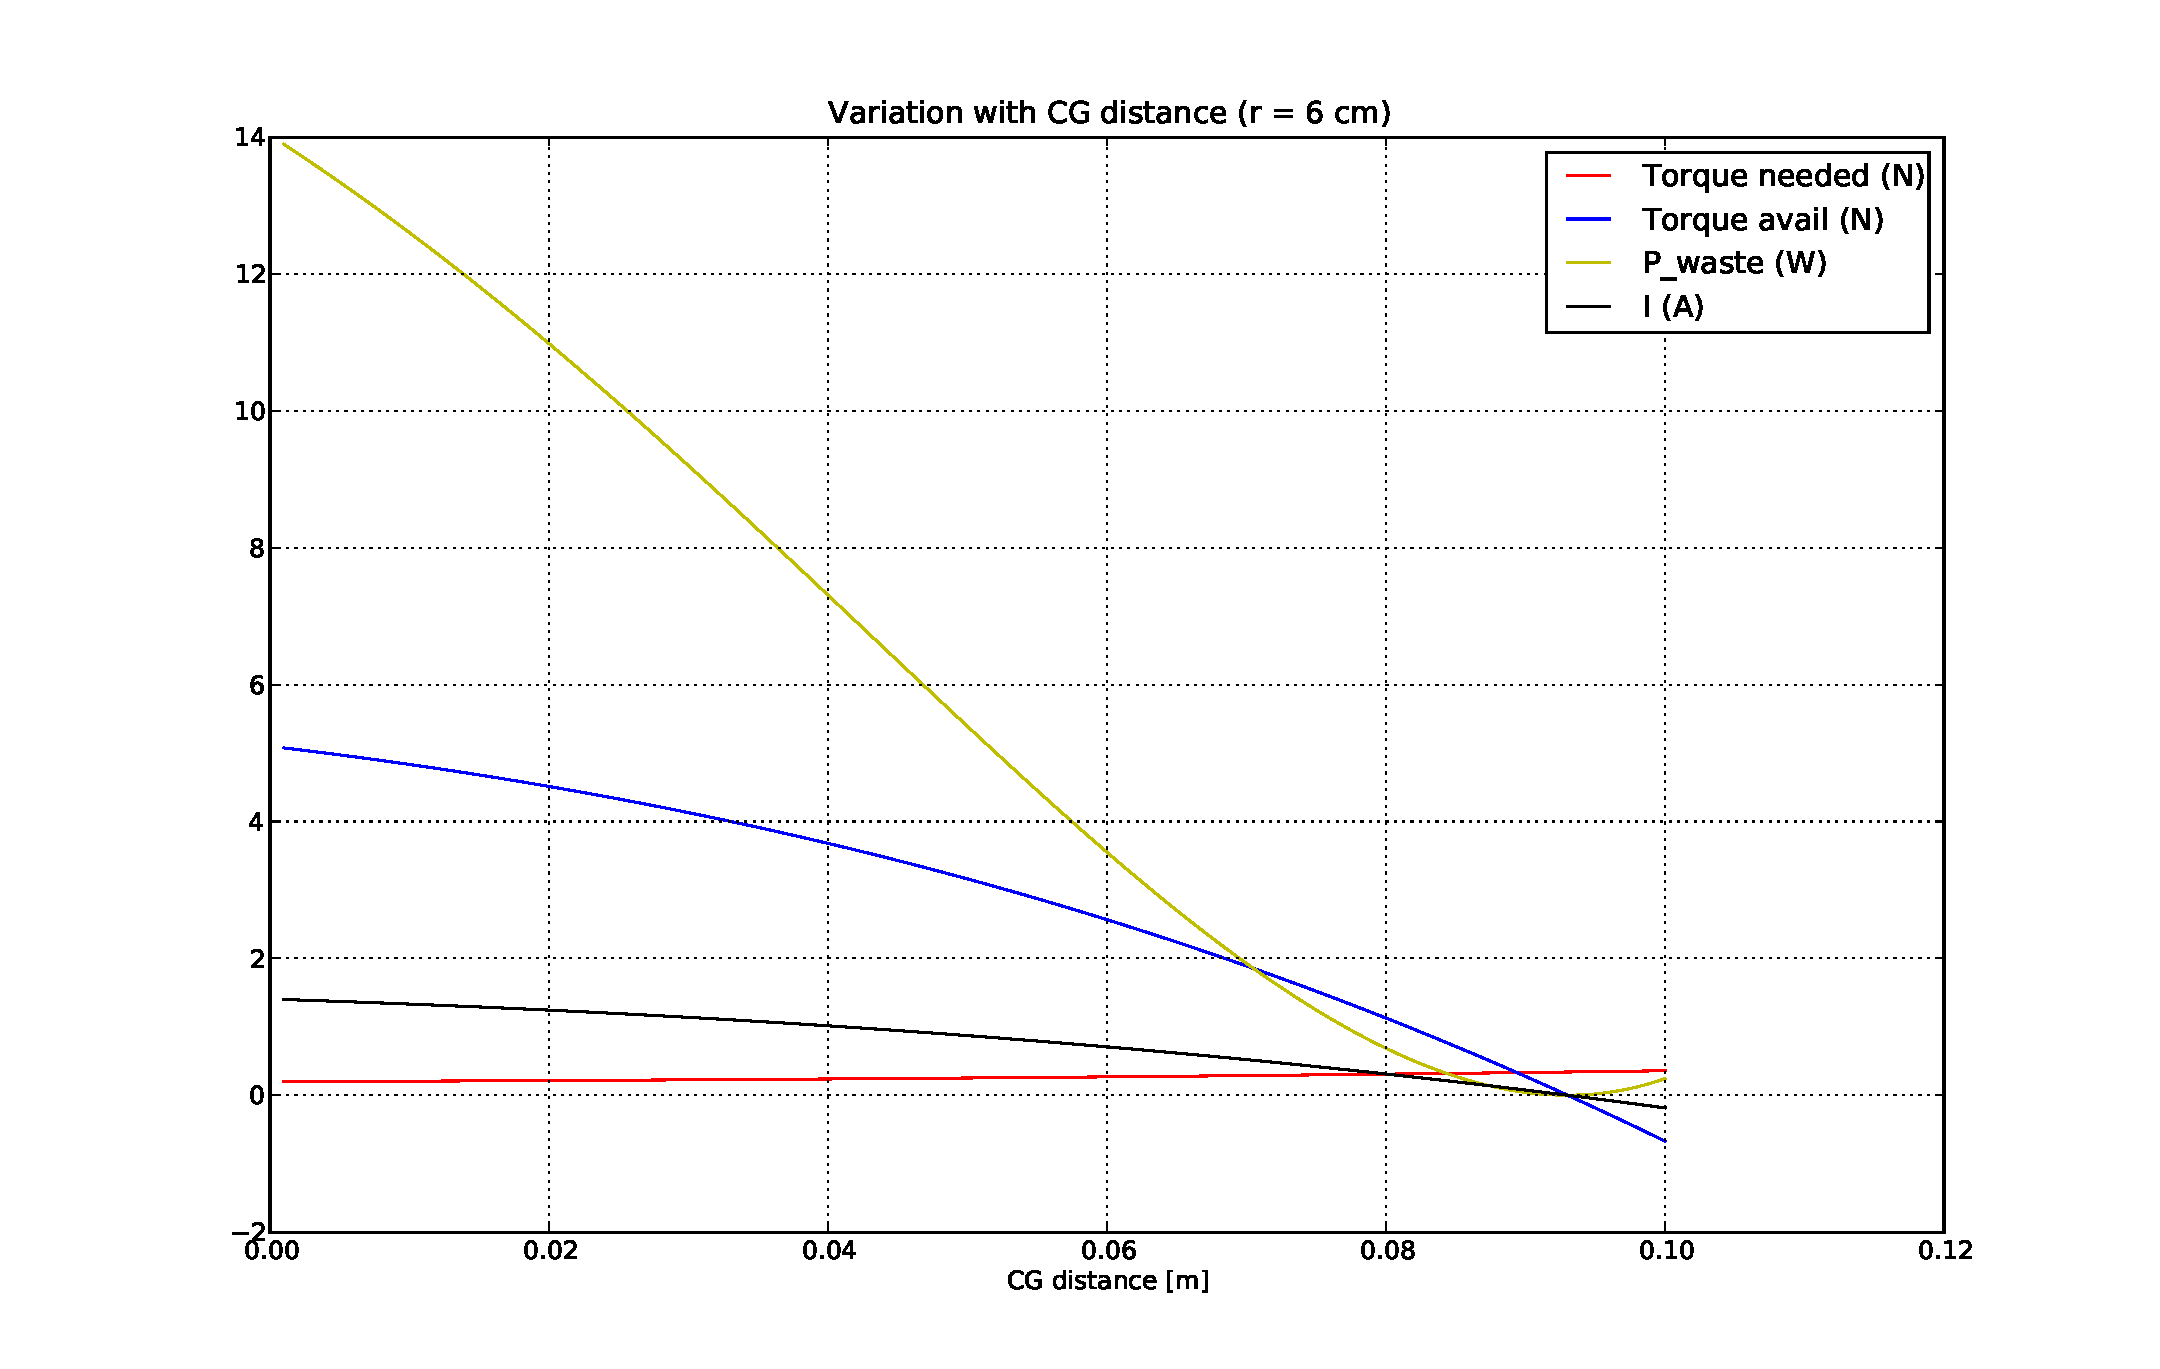
\includegraphics[width=\textwidth]{fig/rewac_dist.pdf}
\end{figure}
\end{frame}

\subsection*{Impact Analysis}
\begin{frame}
\frametitle{Impact Analysis}
\uncover<1->{
\begin{block}{Concept}
\begin{itemize}
\item
Desired hopping height dictates impact frequency\\[0.2in]
\item
Masses dictate energy loss\\[0.2in]
\item
\alert{Natural frequency} of the system should be much \alert{higher} than hopping frequency\\[0.2in]
\end{itemize}
\end{block}
}
\uncover<2->{
\begin{block}{Results}
\begin{itemize}
\item
Hopping frequency is a weak function of hopping height and M\\[0.2in]
\item
\alert{Leg mass} consideration is important
\end{itemize}
\end{block}
}
\end{frame}

\begin{frame}
\frametitle{Impact : Leg mass}
\begin{figure}
\centering
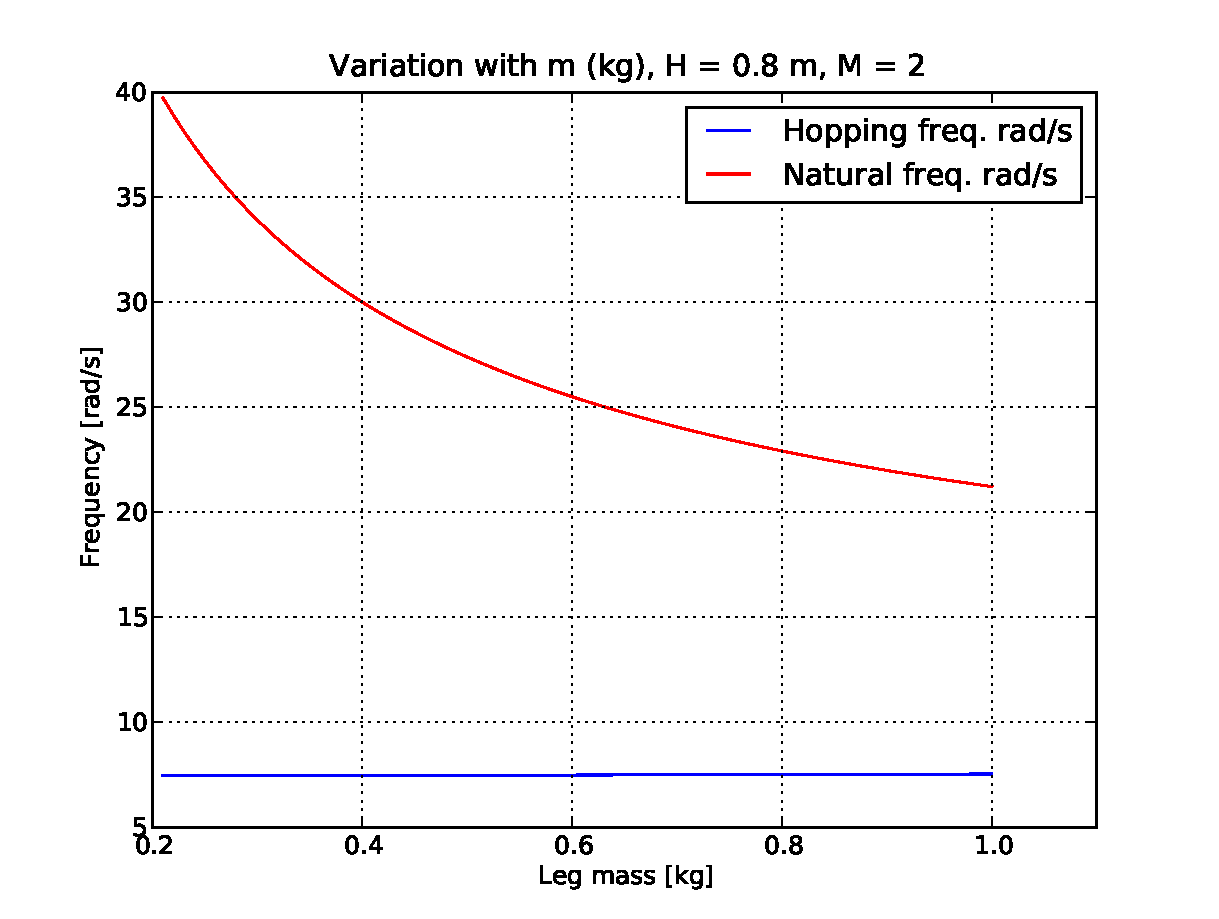
\includegraphics[width=\textwidth]{fig/freq_smallM.pdf}
\end{figure}
\end{frame}

